%chktex-file 46

The eBN is a directed acyclic graph designed to improve traditional BN modeling by incorporating both discrete and continuous events for a more comprehensive probabilistic analysis.
Both eBNs and BNs frameworks, consist of two primary elements: nodes and edges. A node represents an event with its possible determinations and is defined through a Conditional Probability Table (CPT); an edge expresses a direct dependence among 2 nodes, where the originating node is termed the parent.
A node with no incoming edges is referred to as a root node. Nodes that are directly connected by outgoing edges from a given node are called its child nodes.
Non-root nodes have a CPT determined by the combination of all their discrete parents' states.\\

\subsection{eBN main features}
In a traditional BN, each node represents a discrete random variable that can take on a finite number of mutually exclusive and collectively exhaustive states.
For instance, root nodes \textit{A} and  \textit{B}, as well as node \textit{D} in the network depicted in Fig.~\ref{1_ebn_example}, fall into this category.
These nodes are referred to as discrete nodes, and their CPTs are defined using precise probability values, as illustrated in Table~\ref{1_example_CPTs}.
The traditional BN framework is extensively discussed in the work of \textcite{russell_computer}, while its application to reliability analysis is examined in detail in the study by \textcite{langseth_bayesian_2007}.
% These methodologies have been widely adopted in various domains, including risk assessment and decision-making under uncertainty. \\
The eBN framework is capable of handling continuous nodes, which are nodes associated with continuous random variables and consequently, an infinite number of possible states.
The CPT of such nodes is defined using a probability density function (PDF) when the node is a root node, and using a conditional PDF when the node has one or more discrete parents.
For instance, node \textit{C} in Fig.~\ref{1_ebn_example} has a CPT characterized by a univariate normal distribution, $Normal(0,1)$, as illustrated in Table~\ref{1_example_CPTs}. \\  
A node whose CPT is not explicitly defined a priori but instead determined through a model that maps the inputs from its parent nodes to an output generated by the model itself is referred to as a functional node.
The functional nodes can be continuous or discrete. 
In the case of continuous functional nodes, the model alone is sufficient to empirically reconstruct the corresponding CPT.\ 
However for discrete functional nodes, a performance function is required to define their two possible states, which typically represent a failure state and a safe state.
For example, node \textit{M} in Fig.~\ref{1_ebn_example} is a discrete functional node that operates based on this performance function. \\

\begin{figure}[h]
    \centering
    \begin{subfigure}{0.45\textwidth}
        \centering
        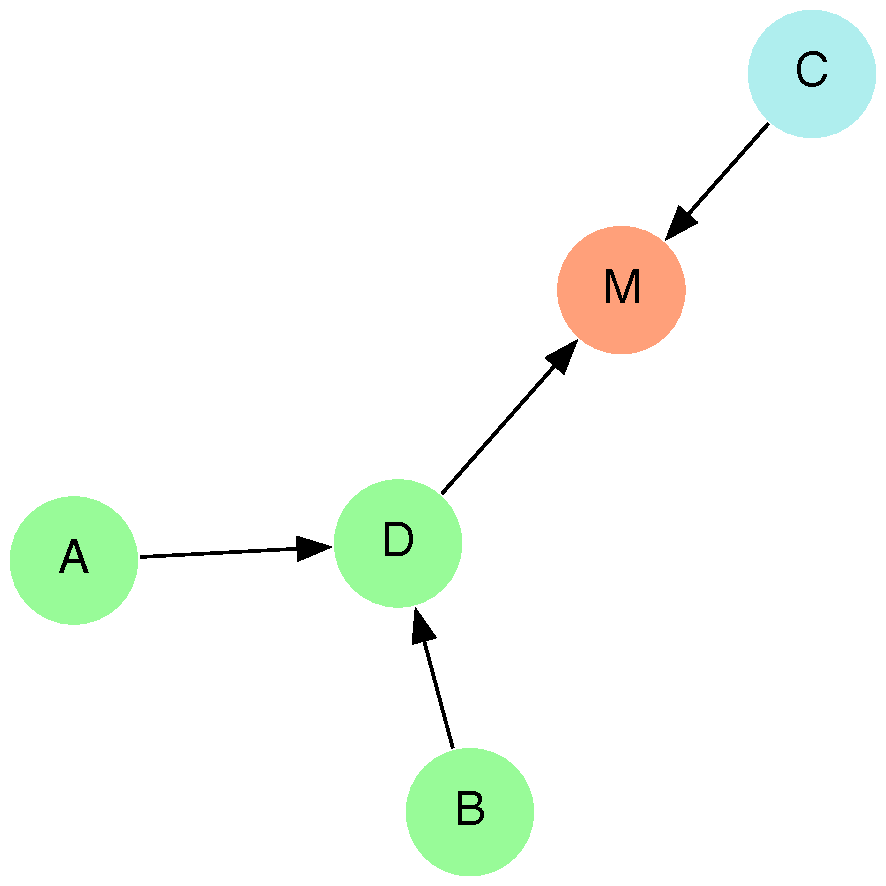
\includegraphics[width=\linewidth]{imgs/pdfs/1_ebn.pdf}
        \caption{Example of an eBN with two discrete root nodes \textit{A} and \textit{B}, one continuous root node \textit{C}, one discrete non-root node \textit{D} and one discrete functional node \textit{M}}\label{1_ebn_example}
    \end{subfigure}
    \hfill
    \begin{subfigure}{0.45\textwidth}
        \centering
        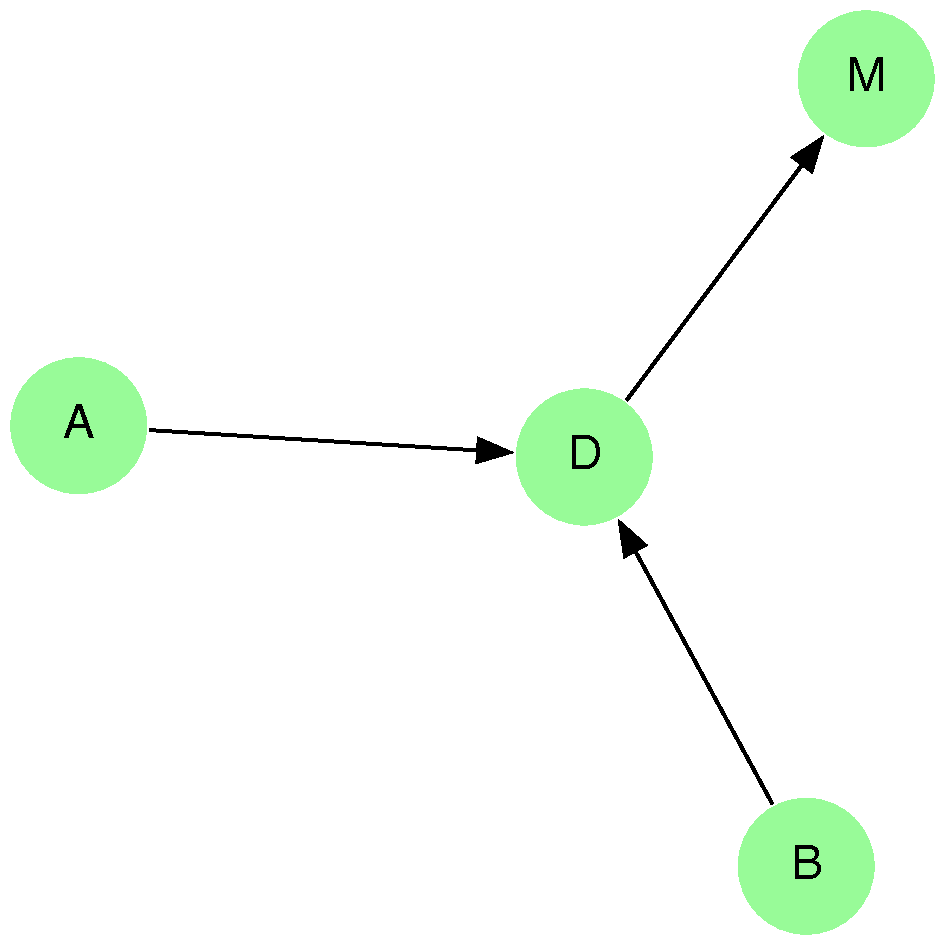
\includegraphics[width=\linewidth]{imgs/pdfs/2_rbn.pdf}
        \caption{Associated rBN where the continuous node \textit{C} is eliminated and the functional nodes \textit{M} is evaluated}\label{1_rbn_example}
    \end{subfigure}
    \caption{Example of reduction of an eBN when no continuous node is discretized}\label{1_reduction_no_disc}
\end{figure}

\begin{table}[!ht]
    \begin{center}
    \caption{CPTs of the eBN}\label{1_example_CPTs}
        \begin{tabular}{P{1.2cm}P{3.9cm}}
            \toprule
            \textbf{Node} & \textbf{CPT} \\
            \midrule
            A & 
                \begin{tabular}{p{0.5cm}p{0.5cm}}
                    \:a1 & \:a2 \\
                    \midrule $0.5$ & $0.5$\\
                \end{tabular}
                \\
                \midrule
            B & 
            \begin{tabular}{p{0.5cm}p{0.5cm}}
                \:b1 & \:b2 \\
                \midrule $0.3$ & $0.7$\\
            \end{tabular}
            \\
            \midrule
            C & $Normal(0;1)$
            \\
            \midrule
            D & 
                \begin{tabular}{p{1.6cm}p{0.5cm}p{0.5cm}}
                    \textbf{scenario} & \:d1 & \:d2 \\
                    \midrule
                    \:a1 \:b1 & $0.6$ & $0.4$ \\
                    \:a1 \:b2 & $0.1$ & $0.9$ \\
                    \:a2 \:b1 & $0.5$ & $0.5$ \\
                    \:a2 \:b2 & $0.5$ & $0.5$ \\
                \end{tabular}
            \\
            \midrule
            M & \begin{tabular}{p{3.3cm}}
                    M:\ $f(d,c) = d - c$ \\
                    P:\ $1-f(d,c) < 0$\\
                \end{tabular}
                \\
        \end{tabular}
    \end{center}
\end{table}

The eBN framework retains the core advantages of traditional BNs, such as the ability to perform multi-scenario analysis, serving as a multidisciplinary aggregator of information, and providing a clear visual representation of complex problems through structured parent-child relationships. 
EBNs further enhance risk assessment capabilities by incorporating aleatoric uncertainties through the inclusion of continuous nodes.
This addition allows for a more robust and realistic representation of uncertain phenomena, thereby improving the model's ability to reflect real-world complexities.\\

Let $\mathbf{Y} = \{Y_1, \ldots, Y_{n_Y}\}$ represent the collection of discrete nodes in the eBN, where each $Y_i$ is a discrete random variable with $k_i$ possible states $\{y_i^1, \ldots, y_i^{k_i}\}$, and let $\mathbf{X} = \{\mathbf{X}_1, \ldots, \mathbf{X}_{n_X}\}$ denote the collection of continuous nodes, where each $\mathbf{X}_i$ is associated with a set of continuous random variables, $\mathbf{X}_i = \{X_{i,1}, \ldots, X_{i,n_i}\}$. 
The joint distribution function of the system can then be expressed through the factorization given in Eq.~\ref{2:factorization_ebn}. 
This mathematical formulation, combined with the application of structural reliability methods (SRMs) to compute joint probability measures in networks with continuous parents, is detailed in the work of \textcite{straub_bayesian_2010}.

\begin{equation}
    \label{2:factorization_ebn}
    p(\mathbf{y}|\mathbf{x})f(\mathbf{x}) = \prod_{Y_i\in \mathbf{Y}} p(y_i|Pa(Y_i)) \prod_{X_i\in \mathbf{X}} f(\mathbf{x}_i|Pa(\mathbf{X}_i)) 
\end{equation}

One of the key strengths of BNs is their ability to utilize exact algorithms to perform \textit{inference} based on available \textit{evidence}, meaning the system's probabilities can be updated given any observed value of a node within the network.
This feature enables BNs to provide accurate and efficient reasoning about uncertain systems. 
% However, in the case of the eBN framework, the application of exact-inference algorithms is not directly feasible due to the inclusion of continuous nodes.
The continuous nature of these nodes complicates the inference process, as they introduce infinite possible states, making traditional exact-inference algorithms inapplicable.  
To address this limitation, once the CPTs for all functional nodes are evaluated, a \textit{node elimination} algorithm, derived from graph theory~\cite{Shachter86a}, is employed. 
This algorithm systematically removes the continuous nodes from the network, while preserving the acyclicity of the eBN at each step, as illustrated in Fig.~\ref{1_reduction_no_disc}. 
By applying this algorithm, the eBN is reduced to a standard BN, which is referred to as the \textit{reduced} BN.\ This reduction allows for the use of well-established exact-inference algorithms for BNs, which enable both prognosis and diagnostic analysis. \\

\begin{figure}[h]
    \centering
    \begin{subfigure}{0.45\textwidth}
        \centering
        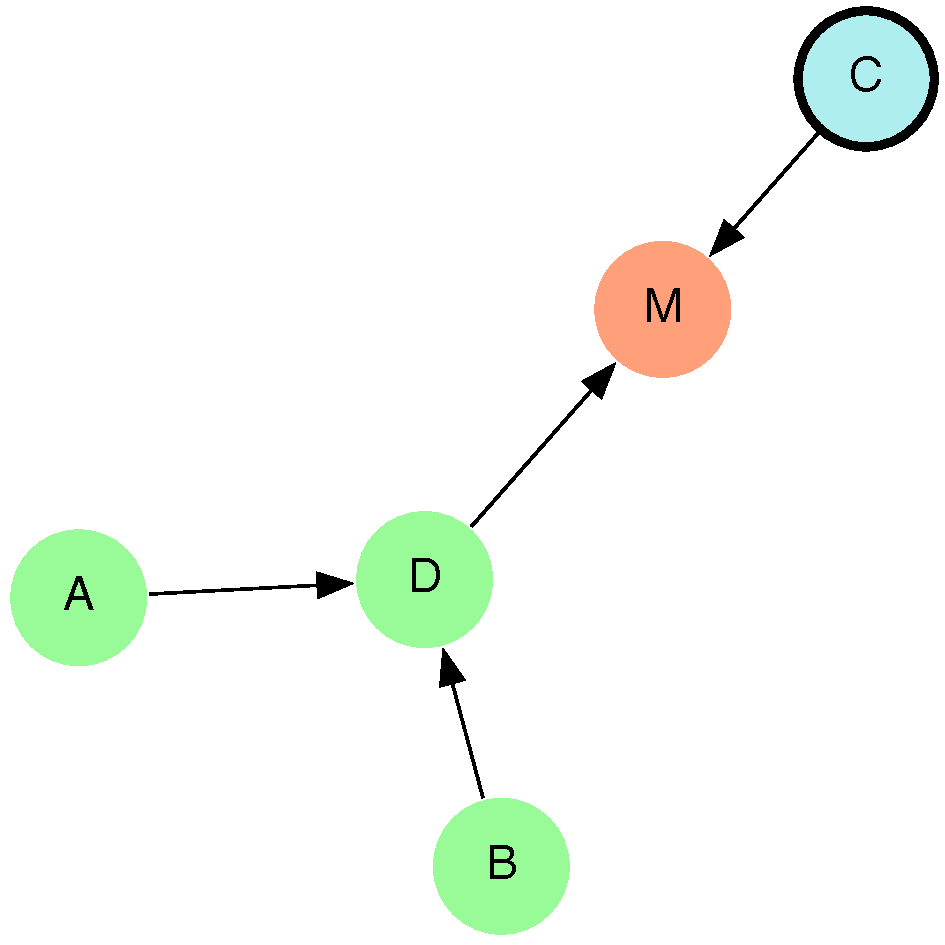
\includegraphics[width=\linewidth]{imgs/pdfs/3_d_ebn.pdf}
        \caption{Example of the same eBN of Fig.\ref{1_ebn_example} with continuous node \textit{C} to be discretized}\label{1_ebn_disc_example}
    \end{subfigure}
    \hfill
    \begin{subfigure}{0.45\textwidth}
        \centering
        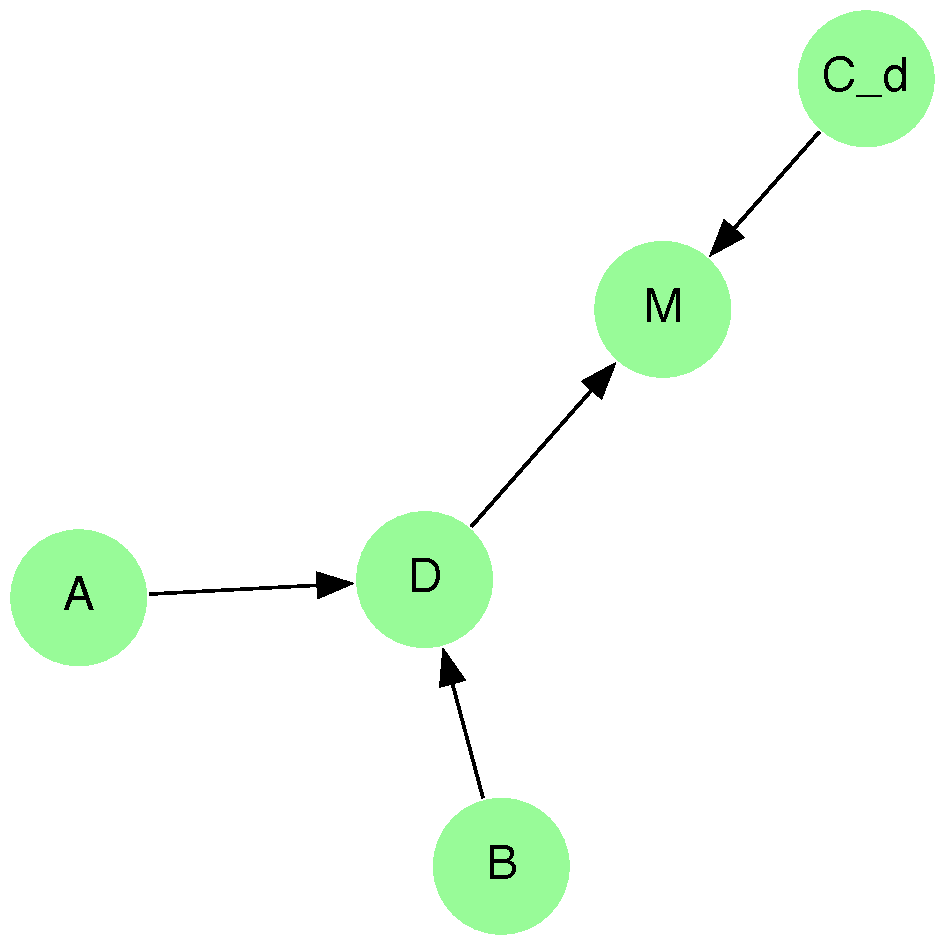
\includegraphics[width=\linewidth]{imgs/pdfs/4_d_rbn.pdf}
        \caption{Associated rBN where the continuous node \textit{C} is discretized into \textit{Cd}}\label{1_rbn_disc_example}
    \end{subfigure}
    \caption{Example of reduction of an eBN when continuous node is discretized}\label{1_reduction_disc}
\end{figure}

\begin{table}[hbt!]
    \begin{center}
        \caption{CPT of the discretized node \textit{Cd} with a $[-3;0;3]$ as discretization interval}\label{exact_disc_tab}
        \begin{tabular}{P{1.5cm}P{1.5cm}P{1.5cm}P{1.5cm}}
            \textbf{$[-\infty;-3]$} & \textbf{$[-3;0]$} & \textbf{$[0;3]$} & \textbf{$[3;\infty]$} \\
            \midrule
            $0.0013499$ & $ 0.49865$ & $ 0.49865$ & $0.0013499$ \\
        \end{tabular}
    \end{center}
\end{table}

\begin{table}[hbt!]
    \begin{center}
        \caption{CPT of the node \textit{M} after being evaluated}\label{Mnode_tab}
        \begin{tabular}{P{2cm}P{2cm}P{2cm}}
            \textbf{scenarios} & \textbf{$M fail$} & \textbf{$M safe$} \\
            \midrule
            $d1;[-\infty;-3]$ & $0$ & $1$ \\
            $d1;[-3;0]$ & $0$ & $1$ \\
            $d1;[0;3]$ & $ 0.48$ & $0.52$ \\
            $d1;[3;+\infty]$ & $ 1$ & $0$ \\
            $d2;[-\infty;-3]$ & $0$ & $1$ \\
            $d2;[-3;0]$ & $0$ & $1$ \\
            $d2;[0;3]$ & $0.79$ & $0.21$ \\
            $d2;[3;+\infty]$ & $1$ & $0$ \\
        \end{tabular}
    \end{center}
\end{table}

Once all continuous nodes have been removed from the network during the network reduction phase, both exact and approximated discretization algorithms can be employed to either consider evidence over these nodes or update their CPTs.
This is shown in Fig.~\ref{1_reduction_disc}, where the continuous node \textit{C} is discretized into the discrete node \textit{Cd}, with the corresponding CPT shown in Tab.~\ref{exact_disc_tab}. 
By discretizing the continuous nodes, it becomes possible to incorporate them into the inference process, allowing for the evaluation of conditional probabilities that involve the former continuous nodes. 
This is illustrated in Tab.~\ref{direct_inference_tab} for the direct inference problem and in Tab.~\ref{inverse_inference_tab} for the inverse inference problem.
Discretization algorithm effectively integrates continuous nodes into the eBN framework, enabling the use of traditional inference techniques while accurately representing aleatoric uncertainty as continuous random variables.\\
Therefore, eBN integrates classical probabilistic modelling with structural reliability methods to form a robust framework for both prognosis and diagnosis across various engineering domains, enhancing decision-making through a more accurate and realistic representation of uncertainty associated with continuous variables. 
% The discretization process ensures that aleatoric uncertainty is effectively captured while preserving the generality of the inference process.\\

\begin{table}[hbt!]
    \begin{center}
        \caption{Direct inference results on node \textit{M} given node $Cd$ state}\label{direct_inference_tab}
        \begin{tabular}{P{3cm}P{3cm}P{3cm}}
            \textbf{evidence} & \textbf{$P(M=fail | Cd)$} & \textbf{$P(M=safe | Cd)$} \\
            \midrule
            $Cd = [-\infty;-3]$ & $0$ & $1$  \\
            $Cd = [-3;0]$ & $0$ & $1$  \\
            $Cd = [0;3]$ & $0.99605$ & $0.00395$ \\
            $Cd = [3;\infty]$ & $0.00395$ & $0.99605$\\
        \end{tabular}
    \end{center}
\end{table}

\begin{table}[hbt!]
    \begin{center}
        \caption{Inverse inference results on node $Cd$ given node \textit{M} in a failure state}\label{inverse_inference_tab}
        \begin{tabular}{P{3cm}P{4cm}}
            \textbf{Query} & \textbf{$P(Query | M = M fail)$} \\
            \midrule
            $Cd = [-\infty;-3]$ & $0$ \\
            $Cd = [-3;0]$ & $0$ \\
            $Cd = [0;3]$ & $0.68305$ \\
            $Cd = [3;\infty]$ & $1$ \\
        \end{tabular}
    \end{center}
\end{table}

\subsection{Imprecise probabilities}
In the current eBN framework, only aleatoric uncertainties are explicitly considered, represented by univariate PDFs, while discrete nodes are assigned crisp probability values. 
However, in real-world applications, both probability distributions and probability assignments often rely on subjective probability, which reflects expert judgments and incomplete or limited data. 
This reliance on subjective probability arises from different factors, such as the inherent unpredictability of some system parameters or the difficulty in obtaining precise data. 
To address this challenge, imprecise probability theory provides a robust and flexible mathematical framework~\cite{beer_imprecise_2013-1} for modelling epistemic uncertainties. 
These uncertainties stem from sources such as conflicting expert opinions, sparse or incomplete datasets, measurement errors, and general knowledge gaps that are common in many engineering and decision-making contexts. 
An eBN that incorporates imprecise probabilities will be referred to as an imprecise eBN throughout the remainder of this paper, enabling more accurate representations of uncertainty in complex systems.

\begin{figure}[h]
    \centering
    \begin{subfigure}{0.45\textwidth}
        \centering
        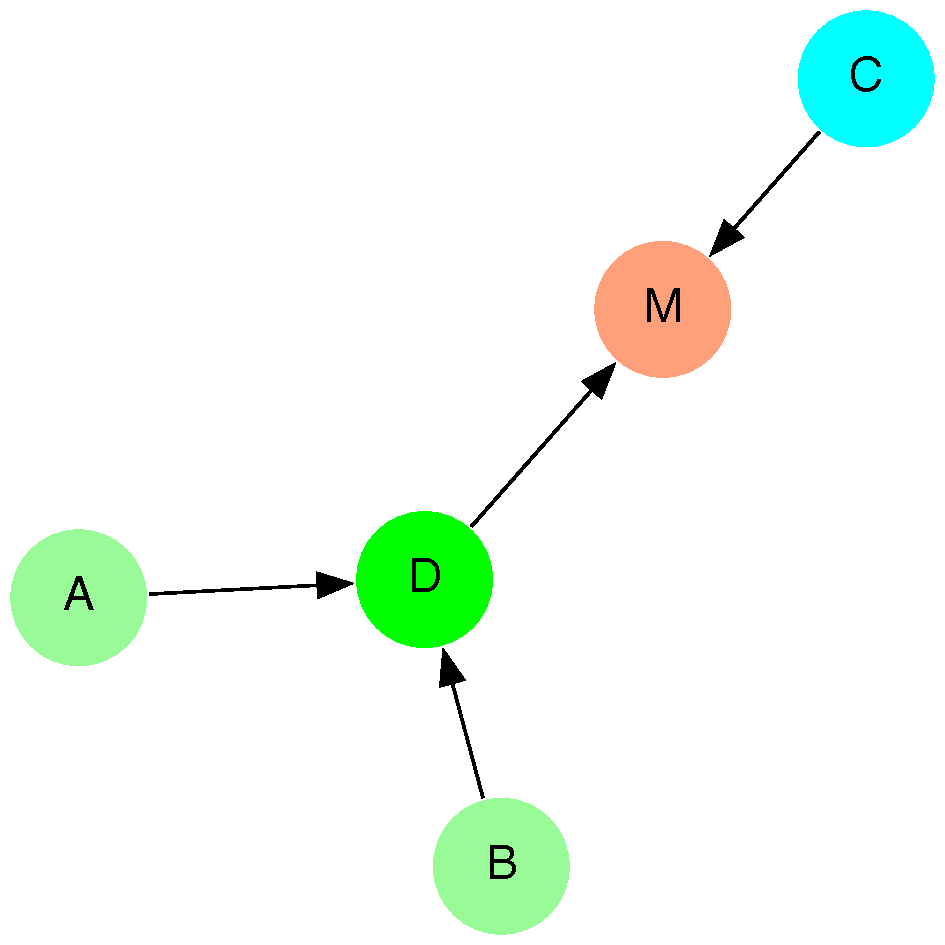
\includegraphics[width=\linewidth]{imgs/pdfs/5_imprecise_ebn.pdf}
        \caption{Example of the same eBN of Fig.\ref{1_ebn_example} but continuous node \textit{C} and discrete node \textit{D} are imprecise}\label{1_imp_ebn}
    \end{subfigure}
    \hfill
    \begin{subfigure}{0.45\textwidth}
        \centering
        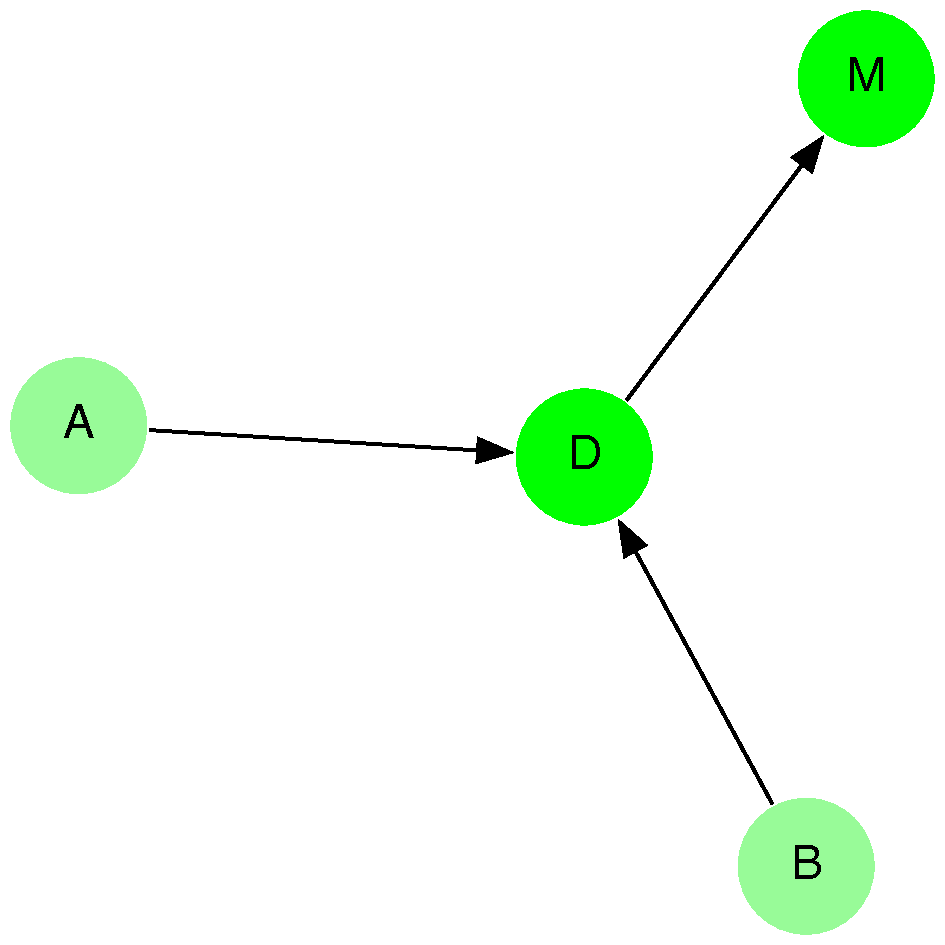
\includegraphics[width=\linewidth]{imgs/pdfs/6_imprecise_rbn.pdf}
        \caption{Associated rBN where model node \textit{M} is imprecise}\label{1_imp_rbn_example}
    \end{subfigure}
    \caption{Example of reduction of eBN with imprecise probabilities}\label{3_imp_reduction}
\end{figure}

\begin{table}[!ht]
    \begin{center}
    \caption{CPTs of the eBN with imprecise probabilities}\label{1_example_CPTs_imprecise}
        \begin{tabular}{P{1.2cm}P{7.8cm}}
            \toprule
            \textbf{Node} & \textbf{CPT} \\
            \midrule
            C & $Pbox\{Normal\}(\mu=[-0.5;0.5];\sigma=[0.8;1.2])$
            \\
            \midrule
            D & 
                \begin{tabular}{P{2.5cm}P{1.5cm}P{1.5cm}}
                    \textbf{scenario} & \:d1 & \:d2 \\
                    \midrule
                    \:a1 \:b1 & $(0.3;0.5)$ & $(0.5;0.7)$ \\
                    \:a1 \:b2 & $(0.0;0.2)$ & $(0.8;1.0)$ \\
                    \:a2 \:b1 & $(0.4;0.6)$ & $(0.4;0.6)$ \\
                    \:a2 \:b2 & $(0.4;0.6)$ & $(0.4;0.6)$ \\
                \end{tabular}
            \\
            \midrule
            M & \begin{tabular}{p{3.3cm}}
                    M:\ $f(d,c) = d - c$ \\
                    P:\ $1-f(d,c) < 0$\\
                \end{tabular}
                \\
        \end{tabular}
    \end{center}
\end{table}

\begin{table}[hbt!]
    \begin{center}
        \caption{CPT of the node \textit{M} after being evaluated in the imprecise eBN}\label{imp_Mnode_tab}
        \begin{tabular}{P{2cm}P{2cm}P{2cm}}
            \textbf{scenarios} & \textbf{$M fail$} & \textbf{$M safe$} \\
            \midrule
            $d1$ & $(0.02;0.6)$ & $(0.4;0.98)$ \\
            $d2$ & $(0.12;0.76)$ & $(0.24;0.88)$ \\
        \end{tabular}
    \end{center}
\end{table}

In the proposed approach, epistemic uncertainties are incorporated into the eBN framework by extending discrete and continuous nodes through imprecise probability theory.
For discrete nodes, the traditionally crisp probability values assigned to each possible state are replaced by probability intervals~\cite{weichselberger_theory_2000}, as demonstrated by node \textit{D} in Fig.~\ref{1_imp_ebn}. 
This replacement captures the inherent uncertainty in probability estimation, reflecting situations where precise probability values cannot be determined. Similarly, for continuous nodes, traditional univariate PDFs are generalized into either probability boxes~\cite{ferson_2003} or probability intervals that refer to the quantity of interest itself, rather than a probability value as seen for discrete nodes. 
For example, node \textit{C} in Fig.~\ref{1_imp_ebn} illustrates this approach, enabling a more flexible representation of uncertainty in continuous distributions.\\

The presence of imprecise nodes, i.e.\ nodes with imprecise CPTs, introduces two main consequences for the analysis of the network. 
First, whenever a continuous node is imprecise, traditional SRMs, such as First Order Reliability Methods (FORM), Monte Carlo simulations, or Advanced Monte Carlo simulations, are no longer directly applicable for evaluating functional nodes. 
Instead, alternative methods, such as DoubleLoop simulation or Random Slicing~\cite{ALVAREZ_randomslicing}, must be employed to appropriately handle the imprecision in continuous variables. 
The presence of imprecise parents for functional nodes means that these nodes are defined by a CPT that includes interval values for both failure and safe state probabilities. In the reduction process shown in Fig.~\ref{3_imp_reduction} nodes CPTs are presented in Tab.~\ref{1_example_CPTs_imprecise} and resulting failure probability interval are the one of Tab.~\ref{imp_Mnode_tab}. 
This approach allows for a more flexible and accurate analysis of systems where uncertainty is present, particularly when dealing with imprecise inputs and uncertain model parameters.

\begin{figure}[H] 
    \centering
    \begin{minipage}{0.5\textwidth} 
        \centering
        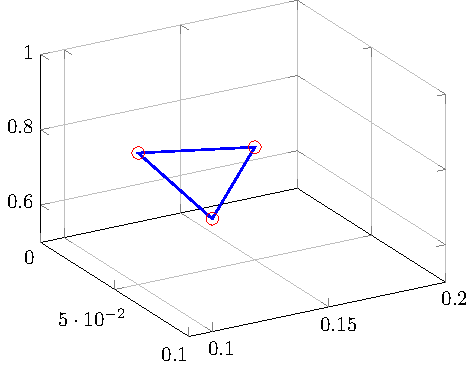
\includegraphics[width=\linewidth]{imgs/pdfs/7_polytope.pdf}
        \caption{Extreme points of the polytope identified by the CPT in Tab.\ref{3_cpt_extremepoints}}\label{3_extreme_points}
    \end{minipage}
    \hfill
    \begin{minipage}{0.4\textwidth}
        \centering
        \begin{tabular}{P{1cm}P{1.5cm}}
            \toprule
            \textbf{states} & \textbf{P} \\
            \midrule
            s1 & $(0.05;0.1)$ \\
            s2 & $(0.1;0.2)$ \\
            s3 & $(0.8;0.9)$ \\
          \end{tabular}
        \captionof{table}{CPT of a discrete imprecise node $S$ with 3 states $s1$, $s2$ and $s3$}\label{3_cpt_extremepoints}
    \end{minipage}
\end{figure}

Whenever a discrete node is imprecise, the rBN is no longer a traditional BN, but instead becomes a Credal Network (CN)~\cite{COZMAN2000199}. 
In the context of CNs, standard exact inference algorithms cannot be directly applied, as the presence of imprecision in the node probabilities introduces a more complex structure. 
To address this, the concept of \textit{strong extension} from the credal set theory~\cite{Levi1980-LEVTEO-7} is employed. 
This extension allows the CN to be decomposed into a set of traditional BNs, each corresponding to one of the extreme points of the n-dimensional polytope in the probability space defined by the intervals of the CPTs of the nodes. This process is illustrated in Fig.~\ref{3_extreme_points}, where each extreme point represents a distinct interpretation of the imprecise probabilities.
Consequently, solving the inference problem for the reduced CN (rCN) of an imprecise eBN requires solving multiple inference problems—one for each extreme point. The result of this process is no longer a single crisp probability value but rather a set of probability bounds, reflecting the uncertainty introduced by the imprecision. This is exemplified in Tab.~\ref{imp_inverse_inference_tab}, which shows the probability bounds for nodes \textit{A} and \textit{B} given that node \textit{M} is in a failure state. These bounds provide a more flexible and robust representation of uncertainty, offering a range of possible outcomes instead of a single deterministic probability, thereby capturing the effects of imprecise information in the network.

\begin{table}[hbt!]
    \begin{center}
        \caption{Inverse inference results on node \textit{A} and \textit{B} given node \textit{M} in a failure state}\label{imp_inverse_inference_tab}
        \begin{tabular}{P{1.5cm}P{4cm}}
            \textbf{Query} & \textbf{$P(Query | M = M fail)$} \\
            \midrule
            $A = a1$ & $(0.281, 0.673)$ \\
            $A = a2$ & $(0.327, 0.719)$ \\
            $B = b1$ & $(0.205, 0.435)$ \\
            $B = b2$ & $(0.565, 0.795)$ \\
        \end{tabular}
    \end{center}
\end{table}

The examples previously discussed, along with the case study and results presented in the following sections, have been implemented using the Julia library \textit{EnhancedBayesianNetworks.jl}~\cite{ebn.jl}.
